% Copyright Luke Olson 2009--2014
% This work is licensed under the Creative Commons
% Attribution-NonCommercial-NoDerivatives 4.0 International License. To view a
% copy of this license, visit http://creativecommons.org/licenses/by-nc-nd/4.0/.
%
\documentclass[10pt]{beamer}
%\documentclass[handout,10pt]{beamer}
%pdflatex -jobname lecture15.print lecture15
%
\mode<presentation>
{
  \usetheme[secheader]{Boadilla}
  \usefonttheme[onlymath]{serif}
  \setbeamercovered{invisible}
  \usecolortheme{luke}
  %\setbeamercovered{transparent}
  %
}
\mode<handout>
{
  \usetheme[secheader]{Boadilla}
  \usefonttheme[onlymath]{serif}
  \setbeamercovered{invisible}
  \usecolortheme{luke2}
  %\setbeamercovered{transparent}
}
\usepackage{pgf,pgfarrows,pgfnodes,pgfautomata,pgfheaps,pgfshade}
\usepackage{pxfonts}
\usepackage{eulervm}
\usepackage{listings}
%\usepackage{pgfpages}
%\pgfpagesuselayout{2 on 1}[letterpaper]
%
%
%%%%%%%%%%%%%%%%%%%%%%%%%%%%%%%%%%%%%%%%%%%%%%%%%%%%%%%%%%%%%%%%%%%%%%%%


%
%
%
\newcommand{\vb}{{\bf{b}}}
\newcommand{\ve}{{\bf{e}}}
\newcommand{\vg}{{\bf{g}}}
\newcommand{\vp}{{\bf{p}}}
\newcommand{\vr}{{\bf{r}}}
\newcommand{\vu}{{\bf{u}}}
\newcommand{\vx}{{\bf{x}}}
\newcommand{\vz}{{\bf{z}}}
\newcommand{\vA}{{\bf{A}}}
\newcommand{\vU}{{\bf{U}}}
\newcommand{\mO}{{\mathcal{O}}}
\newcommand{\mF}{{\mathcal{F}}}
\definecolor{mygray}{rgb}{0.95,0.95,0.95}
\lstset{
        language=matlab,
        numbers=left, numberstyle=\tiny, stepnumber=1, numbersep=5pt,
        basicstyle=\color{black}\ttfamily\small,
        commentstyle=\color{green}\ttfamily,
        keywordstyle=\color{blue}\ttfamily,
        stringstyle=\color{red}\ttfamily,
        showstringspaces=false,
        backgroundcolor=\color{mygray},
        breaklines,
}
\newcommand{\norm}[1]{{\ensuremath{{\|#1\|}}}}
\newcommand{\matdim}[2]{\ensuremath{#1\times#2}}
\newcommand{\rank}[1]{\ensuremath{\mathrm{rank}(#1)}}
\newcommand{\epsm}{\ensuremath{\varepsilon_m}}
\newcommand{\cmd}[1]{{\normalfont\ttfamily\bfseries#1}}

\author{L. Olson}
\institute[UIUC]
{Department of Computer Science\\
University of Illinois at Urbana-Champaign\\
\vspace{0.5cm}
}
%%%%%%%%%%%%%%%%%%%%%%%%%%%%%%%%%%%%%%%%%%%%%%%%%%%%%%%%%%%%%%%%%%%%%%%%
\pgfdeclareimage[height=0.5cm]{university-logo}{./figs/uiuclogo}
\logo{\pgfuseimage{university-logo}}
%%%%%%%%%%%%%%%%%%%%%%%%%%%%%%%%%%%%%%%%%%%%%%%%%%%%%%%%%%%%%%%%%%%%%%%%
\title[CS 357]{Lecture 18}
\subtitle{Integration: Gauss Quadrature}
\date{October 27, 2009}

\begin{document}
% -------------------------------------------------
\begin{frame}
  \titlepage
\end{frame}
% -------------------------------------------------
%%%%%%%%%%%%%%%%%%%%%%%%%%%%%%%%%%%%%%%%%%%%%%%%%%%%%%%%%%%%%%%%%%%%%%%%
\begin{frame}
\frametitle{Today:}
  \begin{block}{Objectives}
    \begin{itemize}
    \item identify the most widely used quadrature method
    \item is it cheap?
    \item is it effective?
    \item how does it compare to Newton-Cotes (Trapezoid, Simpson, etc)?
    \end{itemize}
  \end{block}
  \begin{block}{Material}
    \begin{itemize}
    \item Section 6.2
    \end{itemize}
  \end{block}
\end{frame}
%%%%%%%%%%%%%%%%%%%%%%%%%%%%%%%%%%%%%%%%%%%%%%%%%%%%%%%%%%%%%%%%%%%%%%%%
%%%%%%%%%%%%%%%%%%%%%%%%%%%%%%%%%%%%%%%%%%%%%%%%%%%%%%%%%%%%%%%%%%%%%%%%
\begin{frame}
\frametitle{Quadrature}
\begin{itemize}
  \item up until now, our quadrature methods were of the form
    \begin{equation*}
    \int_a^b f(x)\,dx \approx \sum_{j=0}^{n} w_j f(x_j)
    \end{equation*}
    where $x_j$ are equally spaced nodes
  \item Trapezoid:
    \begin{equation*}
    \int_a^b f(x)\,dx \approx \frac{b-a}{2} f(a) + \frac{b-a}{2} f(b)
    \end{equation*}
  \item Simpson:
    \begin{equation*}
    \int_a^b f(x)\,dx \approx \frac{b-a}{6} f(a) + \frac{2(b-a)}{3}
    f\left(\frac{a+b}{2}\right) + \frac{b-a}{6}f(b)
    \end{equation*}
  \item Similar for higher order polynomial Newton-Cotes rules
\end{itemize}
\end{frame}
%%%%%%%%%%%%%%%%%%%%%%%%%%%%%%%%%%%%%%%%%%%%%%%%%%%%%%%%%%%%%%%%%%%%%%%%%
%%%%%%%%%%%%%%%%%%%%%%%%%%%%%%%%%%%%%%%%%%%%%%%%%%%%%%%%%%%%%%%%%%%%%%%%
\begin{frame}
\frametitle{Quadrature with Freedom}
\begin{alertblock}{!}
  These quadrature rules have one thing in common: they're restrictive
\end{alertblock}
\vspace{0.5cm}

\begin{itemize}
  \item e.g. Simpson:
    \begin{equation*}
    \int_a^b f(x)\,dx \approx \frac{b-a}{6} f(a) + \frac{2(b-a)}{3}
    f\left(\frac{a+b}{2}\right) + \frac{b-a}{6}f(b)
    \end{equation*}
  \item Trapezoid, Simpson, etc (Newton-Cotes) are based on equally spaced
  nodes
\vspace{0.5cm}

  \item We know one thing already from interpolation: equally spaced nodes
  result in \emph{wiggle}.
  \item What other choice do we have?   (...recall how we fixed wiggle in
interpolation: by moving the location of the nodes)
\end{itemize}
\end{frame}
%%%%%%%%%%%%%%%%%%%%%%%%%%%%%%%%%%%%%%%%%%%%%%%%%%%%%%%%%%%%%%%%%%%%%%%%%
%%%%%%%%%%%%%%%%%%%%%%%%%%%%%%%%%%%%%%%%%%%%%%%%%%%%%%%%%%%%%%%%%%%%%%%%
\begin{frame}
\frametitle{Gaussian Quadrature}
  \begin{itemize}
    \item free ourselves from equally spaced nodes
    \item combine selection of the nodes and selection of the weights into
    one quadrature rule
  \end{itemize}
\begin{block}{Gaussian Quadrature}
    Choose the nodes and coefficients optimally to maximize the degree of
precision of the quadrature rule:
    \begin{equation*}
    \int_a^b f(x)\,dx \approx \sum_{j=0}^n w_j f(x_j)
    \end{equation*}
\end{block}
\begin{alertblock}{Goal}
    Seek $w_j$ and $x_j$ so that the quadrature rule is exact for really high polynomials
\end{alertblock}
\end{frame}
%%%%%%%%%%%%%%%%%%%%%%%%%%%%%%%%%%%%%%%%%%%%%%%%%%%%%%%%%%%%%%%%%%%%%%%%%
%%%%%%%%%%%%%%%%%%%%%%%%%%%%%%%%%%%%%%%%%%%%%%%%%%%%%%%%%%%%%%%%%%%%%%%%
\begin{frame}
\frametitle{Gaussian Quadrature}
    \begin{equation*}
    \int_a^b f(x)\,dx \approx \sum_{j=0}^n w_j f(x_j)
    \end{equation*}
  \begin{itemize}
    \item we have $n+1$ points $x_j \,\in\,[a,b]$, $a\le x_0<x_1<\cdots<x_{n-1}<x_n\le b$.
    \item we have $n+1$ real coefficients $w_j$
\vspace{0.5cm}

    \item so there are $2n+2$ total unknowns to take care of
\vspace{0.5cm}

    \item there were only 2 unknowns in the case of trapezoid (2 weights)
    \item there were only 3 unknowns in the case of Simpson (3 weights)
    \item there were only $n+1$ unknowns in the case of general Newton-Cotes
($n+1$ weights)
  \end{itemize}
  \onslide<2->{
  \begin{alertblock}{}
    $2n+2$ unknowns (using $n+1$ nodes) can be used to exactly interpolate and integrate
    polynomials of degree up to $2n+1$
  \end{alertblock}
}
\end{frame}
%%%%%%%%%%%%%%%%%%%%%%%%%%%%%%%%%%%%%%%%%%%%%%%%%%%%%%%%%%%%%%%%%%%%%%%%%
%%%%%%%%%%%%%%%%%%%%%%%%%%%%%%%%%%%%%%%%%%%%%%%%%%%%%%%%%%%%%%%%%%%%%%%%
\begin{frame}
\frametitle{Better Nodes Example}
The first thing we do is SIMPLIFY
  \begin{itemize}
    \item consider the case of $n=1$ (2-point)
    \item consider $[a,b] = [-1,1]$ for simplicity
    \item we \emph{know} how the trapezoid rule works
    \item Question: can we possibly do better using only 2 function evaluations?
    \item Goal: Find $w_0$, $w_1$, $x_0$, $x_1$ so that
    \begin{equation*}
      \int_{-1}^{1} f(x)\, dx \approx w_0 f(x_0) + w_1 f(x_1)
    \end{equation*}
    is as accurate as possible...
  \end{itemize}
\end{frame}
%%%%%%%%%%%%%%%%%%%%%%%%%%%%%%%%%%%%%%%%%%%%%%%%%%%%%%%%%%%%%%%%%%%%%%%%%
%%%%%%%%%%%%%%%%%%%%%%%%%%%%%%%%%%%%%%%%%%%%%%%%%%%%%%%%%%%%%%%%%%%%%%%%
\begin{frame}
\frametitle{Graphical View}
  Consider
    \begin{equation*}
      \int_{1}^{2} x^3 + 1\,dx = 4.75
    \end{equation*}
    \begin{columns}
      \begin{column}{0.45\textwidth}
        \pgfimage[width=5cm]{./figs/quadfig1}
      \end{column}
      \begin{column}{0.45\textwidth}
        \pgfimage[width=5cm]{./figs/quadfig2}
      \end{column}
    \end{columns}
\end{frame}
%%%%%%%%%%%%%%%%%%%%%%%%%%%%%%%%%%%%%%%%%%%%%%%%%%%%%%%%%%%%%%%%%%%%%%%%%
%%%%%%%%%%%%%%%%%%%%%%%%%%%%%%%%%%%%%%%%%%%%%%%%%%%%%%%%%%%%%%%%%%%%%%%%
\begin{frame}
\frametitle{Derive...}
Again, we are considering $[a,b] = [-1,1]$ for simplicity:
\begin{eqnarray*}
  \int_{-1}^1 f(x) \; \mathit{dx} \approx w_0 f(x_0) + w_1 f(x_1)
\end{eqnarray*}
Goal: find $w_0$, $w_1$, $x_0$, $x_1$ so that the approximation is exact up to
cubics.  So try any cubic:
\begin{eqnarray*}
  f(x) = c_0 + c_1 x + c_2 x^2 + c_3 x^3
\end{eqnarray*}
This implies that:
\begin{eqnarray*}
 \int_{-1}^1 f(x) \; \mathit{dx} &=& \int_{-1}^1 \left( c_0 + c_1 x +
 c_2 x^2 + c_3 x^3 \right) \; \mathit{dx} \\
       &=& w_0 \left(c_0 + c_1 x_1 + c_2 x_1^2 + c_3 x_1^3 \right) +   \\
       & & w_1 \left(c_0 + c_1 x_2 + c_2 x_2^2 + c_3 x_2^3 \right) \\
\end{eqnarray*}
\end{frame}
%%%%%%%%%%%%%%%%%%%%%%%%%%%%%%%%%%%%%%%%%%%%%%%%%%%%%%%%%%%%%%%%%%%%%%%%%
\begin{frame}
\frametitle{Derive...}
\begin{eqnarray*}
 \int_{-1}^1 f(x) \; \mathit{dx} &=& \int_{-1}^1 \left( c_0 + c_1 x +
 c_2 x^2 + c_3 x^3 \right) \; \mathit{dx} \\
       &=& w_0 \left(c_0 + c_1 x_1 + c_2 x_1^2 + c_3 x_1^3 \right) +   \\
       & & w_1 \left(c_0 + c_1 x_2 + c_2 x_2^2 + c_3 x_2^3 \right) \\
\end{eqnarray*}
Rearrange into constant, linear, quadratic, and cubic terms:
\begin{eqnarray*}
 c_0 \left(w_0 + w_1 - \int_{-1}^1 \mathit{dx} \right)
&+&  c_1 \left(w_0x_0 + w_1x_1 - \int_{-1}^1 x\;\mathit{dx}
\right)+\\
c_2 \left(w_0x_0^2 + w_1x_1^2 - \int_{-1}^1
x^2\;\mathit{dx}
 \right)
&+&  c_3 \left(w_0x_0^3 + w_1x_1^3 - \int_{-1}^1 x^3\;\mathit{dx}
 \right)  = 0\\
\end{eqnarray*}
Since $c_0$, $c_1$, $c_2$ and $c_3$ are arbitrary, then their
coefficients must all be zero.  
\end{frame}
%%%%%%%%%%%%%%%%%%%%%%%%%%%%%%%%%%%%%%%%%%%%%%%%%%%%%%%%%%%%%%%%%%%%%%%%
\begin{frame}
\frametitle{Derive...}
This implies:
\begin{eqnarray*}
  w_0 + w_1 = \int_{-1}^1 \mathit{dx} = 2 &\qquad&
  w_0x_0 + w_1x_1 = \int_{-1}^1 x\;\mathit{dx} = 0 \\
  w_0x_0^2 + w_1x_1^2 = \int_{-1}^1 x^2\;\mathit{dx} = \frac{2}{3} &\qquad&
  w_0x_0^3 + w_1x_1^3 = \int_{-1}^1 x^3\;\mathit{dx} = 0
\end{eqnarray*}
Some algebra leads to:
\begin{eqnarray*}
  w_0 = 1 \quad w_1 = 1 \quad x_0 = -\frac{\sqrt{3}}{3}
         \quad x_1 = \frac{\sqrt{3}}{3}
\end{eqnarray*}
Therefore:
\begin{eqnarray*}
  \int_{-1}^1 f(x) \; \mathit{dx} \approx f\left(-\frac{\sqrt{3}}{3}
  \right) + f\left(\frac{\sqrt{3}}{3} \right)
\end{eqnarray*}
\end{frame}
%%%%%%%%%%%%%%%%%%%%%%%%%%%%%%%%%%%%%%%%%%%%%%%%%%%%%%%%%%%%%%%%%%%%%%%%%
%%%%%%%%%%%%%%%%%%%%%%%%%%%%%%%%%%%%%%%%%%%%%%%%%%%%%%%%%%%%%%%%%%%%%%%%
\begin{frame}
\frametitle{Over another interval?}
\begin{eqnarray*}
  \int_{-1}^1 f(x) \; \mathit{dx} \approx f\left(-\frac{\sqrt{3}}{3}
  \right) + f\left(\frac{\sqrt{3}}{3} \right)
\end{eqnarray*}
\begin{eqnarray*}
  \int_{a}^b f(x) \; \mathit{dx} \approx ?
\end{eqnarray*}
\begin{itemize}
  \item integrating over $[a,b]$ instead of $[-1,1]$ needs a transformation:
  a change of variables
  \item want $t = c_1 x + c_0$ with $t=-1$ at $x=a$ and $t=1$ at $x=b$
  \item let $ t = \frac{2}{b-a}x-\frac{b+a}{b-a}$
  \item (verify)
  \item let $ x = \frac{b-a}{2}t+\frac{b+a}{2}$
  \item then $dx = \frac{b-a}{2} dt$
\end{itemize}
\end{frame}
%%%%%%%%%%%%%%%%%%%%%%%%%%%%%%%%%%%%%%%%%%%%%%%%%%%%%%%%%%%%%%%%%%%%%%%%
\begin{frame}
\frametitle{Over another interval?}
\begin{eqnarray*}
  \int_{a}^b f(x) \; \mathit{dx} \approx ?
\end{eqnarray*}
\begin{itemize}
  \item let $ x = \frac{b-a}{2}t+\frac{b+a}{2}$
  \item then $dx = \frac{b-a}{2} dt$
  \begin{equation*}
    \int_a^b f(x)\,dx = \int_{-1}^{1}
    f\left(\frac{(b-a)t+b+a}{2}\right)\frac{b-a}{2}\,dt
  \end{equation*}
  \item now use the quadrature formula over $[-1,1]$
  \item note: using two points, $n=1$, gave us exact integration for polynomials of
  degree less 2*1+1 = 3 and less.
\end{itemize}
\end{frame}
%%%%%%%%%%%%%%%%%%%%%%%%%%%%%%%%%%%%%%%%%%%%%%%%%%%%%%%%%%%%%%%%%%%%%%%%%
%%%%%%%%%%%%%%%%%%%%%%%%%%%%%%%%%%%%%%%%%%%%%%%%%%%%%%%%%%%%%%%%%%%%%%%%
\begin{frame}
\frametitle{Extending Gauss Quadrature}
  \begin{itemize}
    \item we need more to make this work for more than two points
    \item A sensible quadrature rule for the interval $[-1,1]$ based on 1
    node would use the node $x=0$.  This is a root of $\phi(x)=x$
    \item Notice: $\pm\frac{1}{\sqrt{3}}$ are the roots of $\phi(x)=3x^2
    -1$
    \item general $\phi(x)$?
  \end{itemize}
\end{frame}
%%%%%%%%%%%%%%%%%%%%%%%%%%%%%%%%%%%%%%%%%%%%%%%%%%%%%%%%%%%%%%%%%%%%%%%%%
%%%%%%%%%%%%%%%%%%%%%%%%%%%%%%%%%%%%%%%%%%%%%%%%%%%%%%%%%%%%%%%%%%%%%%%%%
\begin{frame}
\frametitle{Gauss Quadrature Theorem}
Karl Friedrich Gauss proved the following result:

Let $q(x)$ be a nontrivial polynomial of degree $n+1$ such that
\begin{equation*}
    \int_{a}^{b} x^k q(x) dx = 0 \qquad (0\le k \le n)
\end{equation*}
and let $x_0, x_1, \ldots, x_n$ be the zeros of $q(x)$.  Then
\begin{equation*}
  \int_{a}^{b} f(x)dx \approx \sum_{i=0}^n A_i f(x_i), A_i=\int_{a}^{b} \ell_i(x) dx
\end{equation*}
will be exact for all polynomials of degree at most $2n+1$. (Wow!)
\end{frame}
%%%%%%%%%%%%%%%%%%%%%%%%%%%%%%%%%%%%%%%%%%%%%%%%%%%%%%%%%%%%%%%%%%%%%%%%%
%%%%%%%%%%%%%%%%%%%%%%%%%%%%%%%%%%%%%%%%%%%%%%%%%%%%%%%%%%%%%%%%%%%%%%%%%
\begin{frame}
\frametitle{Sketch of Proof}
Let $f(x)$ be a polynomial of degree $2n+1$.  Then we can write
$f(x) = p(x) q(x) + r(x)$, where $p(x)$ and $r(x)$ are of degree at most $n$ 

(This is basically dividing $f$ by $q$ with remainder $r$).

Then by the hypothesis, $\int_{a}^{b} p(x)q(x)dx = 0$.  Further, 
$f(x_i) = p(x_i)q(x_i) + r(x_i) = r(x_i)$.  Thus, 
\begin{equation*}
   \int_{a}^{b} f(x)dx = \int_{a}^{b} r(x)dx \approx \sum_{i=0}^n f(x_i)\int_{a}^{b}\ell_i(x)dx
\end{equation*}
  But this is exact because $r(x)$ is (at most) a degree $n$ polynomial.

  Thus, we need to find the polynomials $q(x)$.
\end{frame}
%%%%%%%%%%%%%%%%%%%%%%%%%%%%%%%%%%%%%%%%%%%%%%%%%%%%%%%%%%%%%%%%%%%%%%%%%
%%%%%%%%%%%%%%%%%%%%%%%%%%%%%%%%%%%%%%%%%%%%%%%%%%%%%%%%%%%%%%%%%%%%%%%%
\begin{frame}
\frametitle{Orthogonal Polynomials}
  \begin{block}{Orthogonality of Functions}
    Two functions $g(x)$ and $h(x)$ are \emph{orthogonal} on $[a,b]$ if
    \begin{equation*}
      \int_{a}^{b} g(x)h(x)\,dx = 0
    \end{equation*}
  \end{block}
  \begin{itemize}
    \item  so the nodes we're using are roots of orthogonal polynomials
    \item  these are the \emph{Legendre} Polynomials
  \end{itemize}
\end{frame}
%%%%%%%%%%%%%%%%%%%%%%%%%%%%%%%%%%%%%%%%%%%%%%%%%%%%%%%%%%%%%%%%%%%%%%%%%
%%%%%%%%%%%%%%%%%%%%%%%%%%%%%%%%%%%%%%%%%%%%%%%%%%%%%%%%%%%%%%%%%%%%%%%%
\begin{frame}
\framesubtitle{given on the exam}
\frametitle{Legendre Polynomials}
  \begin{align*}
    \phi_0 & = 1\\
    \phi_1 & = x\\
    \phi_2 & = \frac{3x^2-1}{2}\\
    \phi_3 & = \frac{5x^3 - 3x}{2}\\
    \vdots & \\
  \end{align*}
In general:
  \begin{equation*}
    \phi_n(x) = \frac{2n-1}{n} x \phi_{n-1}(x) - \frac{n-1}{n}\phi_{n-2}(x)
  \end{equation*}
\end{frame}
%%%%%%%%%%%%%%%%%%%%%%%%%%%%%%%%%%%%%%%%%%%%%%%%%%%%%%%%%%%%%%%%%%%%%%%%%
%%%%%%%%%%%%%%%%%%%%%%%%%%%%%%%%%%%%%%%%%%%%%%%%%%%%%%%%%%%%%%%%%%%%%%%%
\begin{frame}
\frametitle{Notes on Legendre Roots}
\vspace{-0.5cm}
\begin{center}
  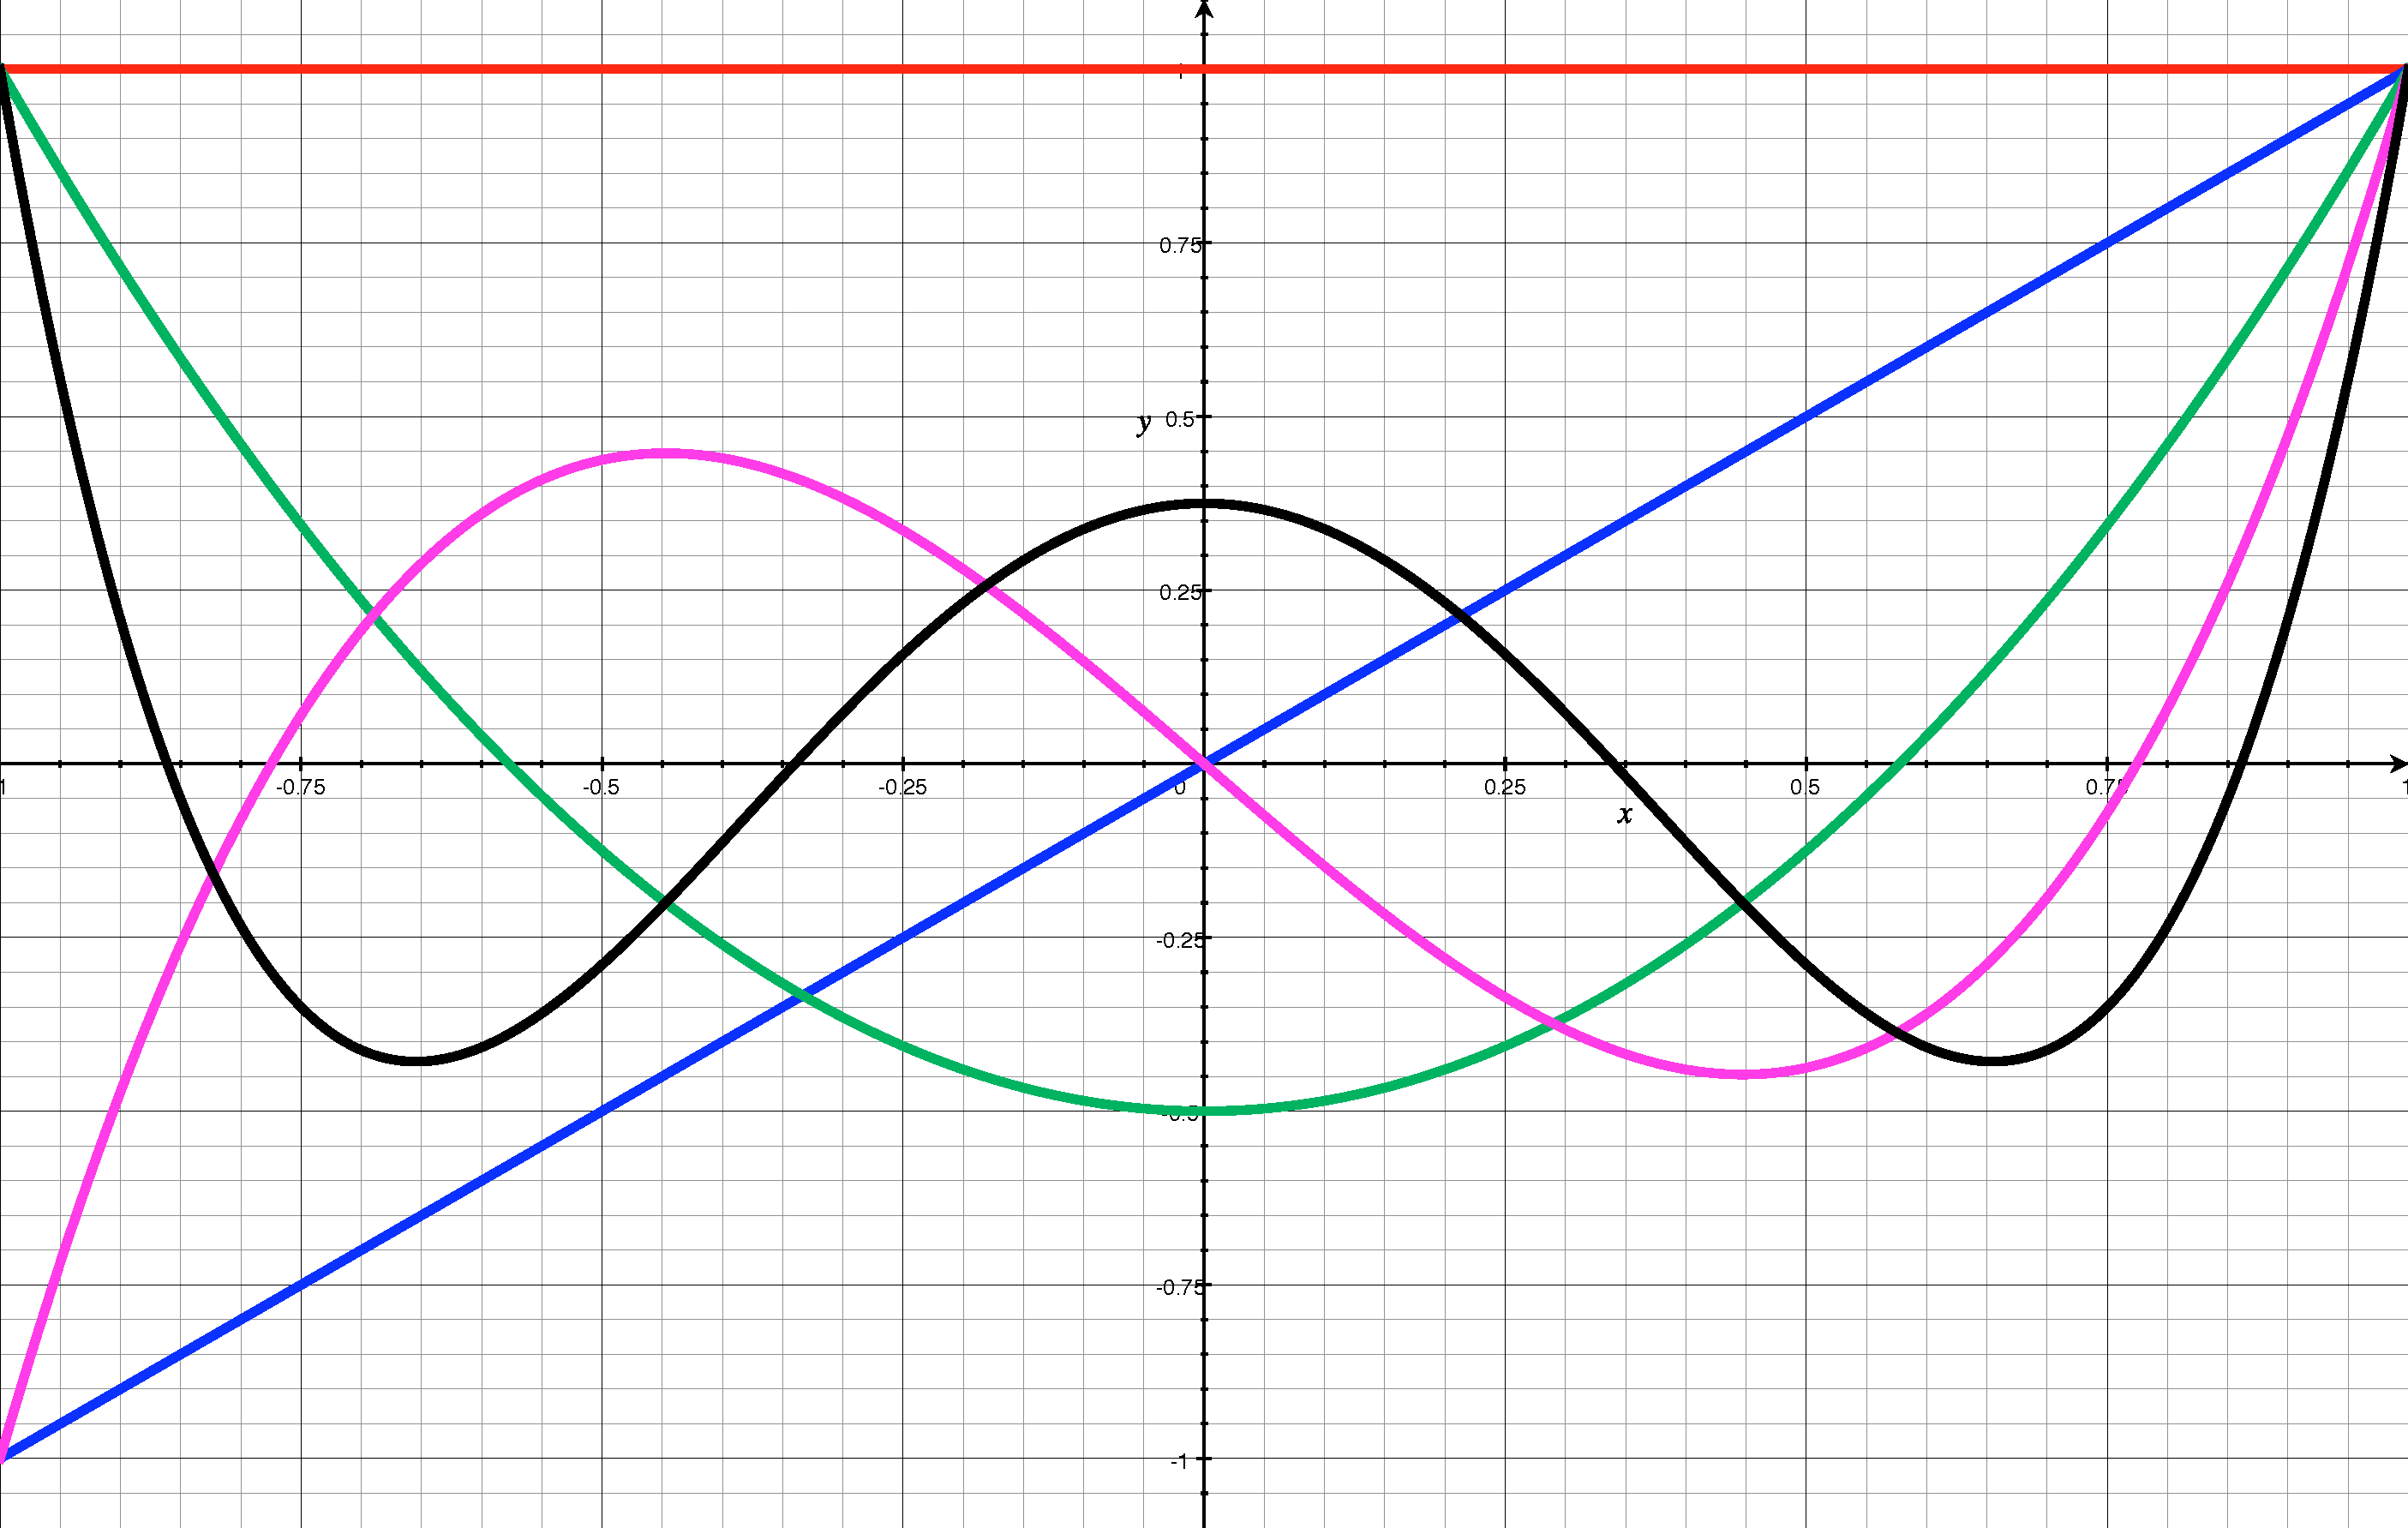
\includegraphics[height=3.5cm]{./figs/legendre.pdf}
\end{center}
  \begin{itemize}
    \item The Legendre Polynomials are orthogonal (nice!)
    \item The Legendre Polynomials increase in polynomials order (like
    monomials)
    \item The Legendre Polynomials don't suffer from poor conditioning (unlike
    monomials...more in the linear algebra section)
    \item The Legendre Polynomials don't have a closed form expression
    (recursion relation is needed)
    \item The roots of the Legendre Polynomials are the nodes for Gaussian
    Quadrature (GL nodes)
  \end{itemize}
\end{frame}
%%%%%%%%%%%%%%%%%%%%%%%%%%%%%%%%%%%%%%%%%%%%%%%%%%%%%%%%%%%%%%%%%%%%%%%%%
%%%%%%%%%%%%%%%%%%%%%%%%%%%%%%%%%%%%%%%%%%%%%%%%%%%%%%%%%%%%%%%%%%%%%%%%
\begin{frame}[containsverbatim,shrink]
\frametitle{Quadrature Nodes (see) }
\begin{itemize}
  \item Often listed in tables
  \item Weights determined by extension of above
  \item Roots are symmetric in $[-1,1]$
  \item Example:
  \begin{lstlisting}
  if(n==0)
    x = 0;   w = 2;
  if(n==1)
    x(1) = -1/sqrt(3);     x(2) = -x(1);
    w(1) =  1;             w(2) =  w(1);
  if(n==2)
    x(1) = -sqrt(3/5);    x(2) =  0;      x(3) = -x(1);
    w(1) =  5/9;          w(2) =  8/9;    w(3) =  w(1);
  if(n==3)
    x(1) = -0.861136311594053;     x(4) = -x(1);
    x(2) = -0.339981043584856;     x(3) = -x(2);
    w(1) =  0.347854845137454;     w(4) =  w(1);
    w(2) =  0.652145154862546;     w(3) =  w(2);
  if(n==4)
    x(1) = -0.906179845938664;     x(5) = -x(1);
    x(2) = -0.538469310105683;     x(4) = -x(2);
    x(3) =  0;
    w(1) =  0.236926885056189;     w(5) =  w(1);
    w(2) =  0.478628670499366;     w(4) =  w(2);
    w(3) =  0.568888888888889;
  if(n==5)
    x(1) = -0.932469514203152;     x(6) = -x(1);
    x(2) = -0.661209386466265;     x(5) = -x(2);
    x(3) = -0.238619186083197;     x(4) = -x(3);
    w(1) =  0.171324492379170;     w(6) =  w(1);
    w(2) =  0.360761573048139;     w(5) =  w(2);
    w(3) =  0.467913934572691;     w(4) =  w(3);
  \end{lstlisting}
\end{itemize}
\end{frame}
%%%%%%%%%%%%%%%%%%%%%%%%%%%%%%%%%%%%%%%%%%%%%%%%%%%%%%%%%%%%%%%%%%%%%%%%%
%%%%%%%%%%%%%%%%%%%%%%%%%%%%%%%%%%%%%%%%%%%%%%%%%%%%%%%%%%%%%%%%%%%%%%%%
\begin{frame}
\frametitle{View of Nodes}
\begin{center}
  \pgfimage[width=7.5cm]{./figs/GaussNodes}
\end{center}
\end{frame}
%%%%%%%%%%%%%%%%%%%%%%%%%%%%%%%%%%%%%%%%%%%%%%%%%%%%%%%%%%%%%%%%%%%%%%%%
\begin{frame}
\frametitle{Theory}
The connection between the roots of the Legendre polynomials and
exact integration of polynomials is established by the following
theorem.

\begin{block}{Theorem} Suppose that $x_0, x_1, \ldots, x_n$ are roots of
the $n$th Legendre polynomial $P_n(x)$ and that for each $i = 0,1,
\ldots, n$ the numbers $w_i$ are defined by
$$w_i = \int_{-1}^1 \prod^n_{\small \begin{array}{c}
  j=0 \\
  j \ne i\\
\end{array}
} \frac{x-x_j}{x_i - x_j}dx = \int_{-1}^{1} \ell_i(x)\,dx
$$

Then 
$$\int_{-1}^1 f(x)dx = \sum_{i=0}^n w_i f(x_i),$$
where $f(x)$ is any polynomial of degree less or equal to $2n+1$.
\end{block}
\end{frame}
%%%%%%%%%%%%%%%%%%%%%%%%%%%%%%%%%%%%%%%%%%%%%%%%%%%%%%%%%%%%%%%%%%%%%%%%%
%%%%%%%%%%%%%%%%%%%%%%%%%%%%%%%%%%%%%%%%%%%%%%%%%%%%%%%%%%%%%%%%%%%%%%%%
\begin{frame}
\frametitle{Do not!}
\begin{alertblock}{!!!}
When evaluating a quadrature rule
\begin{equation*}\int_{-1}^1 f(x)dx = \sum_{i=0}^n w_i f(x_i).\end{equation*}
\emph{do not} generate the nodes and weights each time.  Use a lookup
table...
\end{alertblock}
\end{frame}
%%%%%%%%%%%%%%%%%%%%%%%%%%%%%%%%%%%%%%%%%%%%%%%%%%%%%%%%%%%%%%%%%%%%%%%%%
%%%%%%%%%%%%%%%%%%%%%%%%%%%%%%%%%%%%%%%%%%%%%%%%%%%%%%%%%%%%%%%%%%%%%%%%
\begin{frame}
\frametitle{Example}
Approximate $\displaystyle \int_1^{1.5} x^2\ln x ~dx$ using
Gaussian quadrature with $n=1$. \\
\underline{\textsc{Solution}} As derived earlier we want to use $
\displaystyle \int_{-1}^1 f(x) \; \mathit{dx} \approx
f\left(-\frac{\sqrt{3}}{3}
  \right) + f\left(\frac{\sqrt{3}}{3} \right)$ \\
From earlier we know that we are interested in
\begin{eqnarray*}
  \int_1^{1.5} f(x) \; \mathit{dx} = \int_{-1}^1 f\left(\frac{(1.5-1)t+(1.5+1)}{2}\right) \;
  \frac{1.5-1}{2} \; \mathit{dt}
\end{eqnarray*}
Therefore, we are looking for the integral of
$$\frac{1}{4}\int_{-1}^1 f\left(\frac{x+5}{4}\right)
dx = \frac{1}{4}\int_{-1}^1  \left(\frac{x+5}{4}\right)^2
\ln\left(\frac{x+5}{4}\right)dx
$$
Using Gaussian quadrature, our numerical integration becomes:
$$\frac{1}{4}\left[\left(\frac{-\frac{\sqrt{3}}{3}+5}{4}\right)^2 \ln\left(\frac{-\frac{\sqrt{3}}{3}+5}{4}\right)
+ \left(\frac{\frac{\sqrt{3}}{3}+5}{4}\right)^2
\ln\left(\frac{\frac{\sqrt{3}}{3}+5}{4}\right) \right] =
0.1922687
$$
\end{frame}
%%%%%%%%%%%%%%%%%%%%%%%%%%%%%%%%%%%%%%%%%%%%%%%%%%%%%%%%%%%%%%%%%%%%%%%%%
%%%%%%%%%%%%%%%%%%%%%%%%%%%%%%%%%%%%%%%%%%%%%%%%%%%%%%%%%%%%%%%%%%%%%%%%
\begin{frame}
\frametitle{Example}
Approximate $\displaystyle \int_0^{1} x^2 e^{-x} ~dx$ using
Gaussian quadrature with $n=1$. \\
\underline{\textsc{Solution}} We again want to convert our limits
of integration to -1 to 1. Using the same process as the earlier
example, we get:
$$\int_0^1 x^2 e^{-x} dx = \frac{1}{2}\int_{-1}^1 \left(
\frac{t+1}{2}\right)^2 e^{(t+1)/2}dt.$$ Using the Gaussian roots
we get:
$$\int_0^1 x^2 e^{-x} dx \approx \frac{1}{2}\left[\left(\frac{-\frac{\sqrt{3}}{3}+1}{2}\right)^2 e^{(-\frac{\sqrt{3}}{3}+1)/2}
+ \left(\frac{\frac{\sqrt{3}}{3}+1}{2}\right)^2
e^{(\frac{\sqrt{3}}{3}+1)/2} \right] = 0.1594104$$
\end{frame}
%%%%%%%%%%%%%%%%%%%%%%%%%%%%%%%%%%%%%%%%%%%%%%%%%%%%%%%%%%%%%%%%%%%%%%%%%
\begin{frame}
\begin{block}{Numerical Question}
How does $n$ point Gauss quadrature compare with $n$ point Newton-Cotes...
\end{block}
\end{frame}
%%%%%%%%%%%%%%%%%%%%%%%%%%%%%%%%%%%%%%%%%%%%%%%%%%%%%%%%%%%%%%%%%%%%%%%%
\begin{frame}[shrink]
\frametitle{Examples}
\framesubtitle{with matlab...}
\begin{example}
  int\_gauss.m:  base routine for Gauss quadrature
\end{example}
\begin{example}
  int\_gauss\_test.m: integrate $\int_{0}^{5} x e^{-x}\,dx$ with
  \begin{enumerate}
    \item 1 subinterval, increasing number of nodes
    \item 3 nodes, increases number of intervals (panels)
  \end{enumerate}
  Result: fewer total evaluations in GL quadrature with 1 subinterval and many
  nodes versus 3 nodes and many subpanels.  Also more accurate.
\end{example}
\begin{example}
  int\_compare\_gauss\_trapezoid\_simpson.m: integrate $\int_{0}^{5} x e^{-x}\,dx$ with
  \begin{enumerate}
    \item trapezoid
    \item Simpson
    \item Gauss
  \end{enumerate}
  Keep the number of number of nodes and panels consistent.  Result: fewer evals
for Gauss
\end{example}
\end{frame}
%%%%%%%%%%%%%%%%%%%%%%%%%%%%%%%%%%%%%%%%%%%%%%%%%%%%%%%%%%%%%%%%%%%%%%%%%
\begin{frame}
\frametitle{Something interesting...}
  \begin{center}
  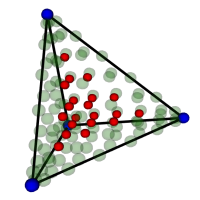
\includegraphics[height=4cm]{./figs/tet}
  \end{center}
\begin{itemize}
  \item Gauss nodes in other shapes are not easy
  \item One approach: let electrostatics determine the (uneven) distribution
\end{itemize}
\end{frame}
%%%%%%%%%%%%%%%%%%%%%%%%%%%%%%%%%%%%%%%%%%%%%%%%%%%%%%%%%%%%%%%%%%%%%%%%
%%%%%%%%%%%%%%%%%%%%%%%%%%%%%%%%%%%%%%%%%%%%%%%%%%%%%%%%%%%%%%%%%%%%%%%%
\begin{frame}
\frametitle{Quadrature}
\begin{center}
  \pgfimage[width=0.8\textwidth]{./figs/brick1}
\end{center}
\end{frame}
%%%%%%%%%%%%%%%%%%%%%%%%%%%%%%%%%%%%%%%%%%%%%%%%%%%%%%%%%%%%%%%%%%%%%%%%
%%%%%%%%%%%%%%%%%%%%%%%%%%%%%%%%%%%%%%%%%%%%%%%%%%%%%%%%%%%%%%%%%%%%%%%%
\begin{frame}
\frametitle{Quadrature}
\begin{center}
  \pgfimage[width=0.8\textwidth]{./figs/brick2}
\end{center}
40K tetrahedrons.
\end{frame}
%%%%%%%%%%%%%%%%%%%%%%%%%%%%%%%%%%%%%%%%%%%%%%%%%%%%%%%%%%%%%%%%%%%%%%%%
%%%%%%%%%%%%%%%%%%%%%%%%%%%%%%%%%%%%%%%%%%%%%%%%%%%%%%%%%%%%%%%%%%%%%%%%
\begin{frame}
\frametitle{Quadrature}
\begin{columns}
\begin{column}{0.45\textwidth}
\begin{center}
  \pgfimage[width=5cm]{./figs/brick2}
\end{center}
\end{column}
\begin{column}{0.45\textwidth}
\begin{center}
  \pgfimage[width=3cm]{./figs/tetrahedron}
\end{center}
\end{column}
\end{columns}
\begin{itemize}
  \item 40K tetrahedrons.
  \item need to integrate a function $f(x)$ over each tet $\Omega_i$: $\int_{\Omega_i} f(x)\,dx$
  \item needs quadrature
  \item map the integration to a reference tetrahedron
  \item perform Gauss Quadrature using $(n+1)(n+2)(n+3)/6$ quadrature
points (where $n$ is the 1-D number of points).
  \item $f(x)$ is often a product of degree $m$ Lagrange interpolating
polynomials
  \item ...needs large $n$
  \item results in \# of tetrahedrons $\times$ $n^3/6$ function evaluations
\end{itemize}
\end{frame}
%%%%%%%%%%%%%%%%%%%%%%%%%%%%%%%%%%%%%%%%%%%%%%%%%%%%%%%%%%%%%%%%%%%%%%%%
\end{document}
